% ============================================================================
%  CK0475 — APRESENTAÇÃO FINAL · dosimeter-mg24
%  Marcelo Correa (mat. 510181) · UFC 2026.2 · Prof. Cesar Lincoln C. Mattos
%
%  Todos os números medidos vêm de docs/03-development/MEASURED-2026-11-17.md,
%  lidos da placa XIAO MG24 Sense (2886:0062:28DB6336) pelo mailbox e pelo
%  cycle counter. O que não foi medido aparece como [A MEDIR] — nunca como zero.
% ============================================================================
\documentclass[aspectratio=169,10pt]{beamer}
\usetheme{Madrid}
\usecolortheme{seahorse}

\usepackage[utf8]{inputenc}
\usepackage[T1]{fontenc}
\usepackage[brazilian]{babel}
\usepackage{booktabs}
\usepackage{graphicx}
\usepackage{siunitx}

\title[Dosímetro com incerteza]{Dosímetro de ruído com incerteza}
\subtitle{Um sensor acústico que diz quanto vale a sua previsão}
\author{Marcelo Correa · mat.\ 510181}
\institute[UFC]{Universidade Federal do Ceará · CK0475 Aprendizagem de Máquina Probabilística}
\date{Novembro de 2026}

\begin{document}

\begin{frame}
  \titlepage
\end{frame}

\begin{frame}{O problema: um número não é uma decisão}
  \begin{block}{NR-15}
    Limite de \SI{85}{\decibel} para 8 horas; taxa de troca de \SI{5}{\decibel} — cada
    \SI{5}{\decibel} a mais divide o tempo admissível por dois.
  \end{block}
  \vspace{0.3cm}
  \begin{alertblock}{Porque a incerteza muda a decisão}
    \SI{84}{\decibel} $\pm \SI{1.5}{\decibel}$: limite não excedido com confiança.\\
    \SI{88}{\decibel} $\pm \SI{6}{\decibel}$: \textbf{não se sabe} — é preciso medir mais.
  \end{alertblock}
  \vspace{0.2cm}
  Um dosímetro comercial devolve o primeiro tipo de número nos dois casos.
\end{frame}

\begin{frame}{Aplicabilidade}
  \begin{enumerate}
    \item \textbf{Dosímetro pessoal} — saúde ocupacional; o intervalo diz se o limite foi
          excedido ou se a medição é insuficiente.
    \item \textbf{Anomalias em máquinas} — um microfone por máquina numa oficina; a densidade
          aprendida detecta o som novo.
    \item \textbf{Rede de nós urbanos} — sensores baratos sem sincronismo entre si; cada um
          reporta nível e incerteza quando um telemóvel passa.
  \end{enumerate}
  \vspace{0.3cm}
  \footnotesize Nota de desenho: um dosímetro é, por natureza, um dispositivo de \emph{um}
  microfone — dois seriam um luxo que ninguém leva ao colete.
\end{frame}

\begin{frame}{O hardware que mediu isto}
  \begin{columns}[T]
    \begin{column}{0.52\textwidth}
      \begin{itemize}
        \item XIAO MG24 Sense — Cortex-M33
        \item Microfone MEMS \textbf{na placa} (PC9, ADC 12 bits)
        \item BLE (GATT verificado com telemóvel)
        \item MVP — acelerador de matrizes/vetores
        \item Alvo: Rust \texttt{no\_std}, sem alocador
      \end{itemize}
    \end{column}
    \begin{column}{0.44\textwidth}
      \begin{block}{Porque este hardware}
        Sem fios externos: não há módulo que avarie, nem soldadura a falhar.\\
        O modelo corre no dispositivo — não se envia áudio por rádio.
      \end{block}
    \end{column}
  \end{columns}
\end{frame}

\begin{frame}{Primeira medição: a taxa do microfone}
  \begin{block}{Medido na placa (não é datasheet)}
    \textbf{\num{303148} amostras/s}, \SI{62.7}{ciclos} por amostra, conversões polled.\\
    Duas corridas independentes: \num{303148} e \num{303149} amostras em \num{19000068} e
    \num{19000056} ciclos.
  \end{block}
  \vspace{0.2cm}
  \begin{alertblock}{O que isto custa}
    \SI{11.47}{M} ciclos/s = \textbf{\SI{60.4}{\percent} do núcleo} só a pedir amostras.
  \end{alertblock}
  \vspace{0.2cm}
  \footnotesize Causa de um defeito anterior: \texttt{GPIO\_CDBUSALLOC.CDODD0} nunca foi escrito,
  PC9 nunca chegou ao ADC0, e o conversor devolvia zero — que \texttt{level()} reportava como
  \texttt{rms=2048}.
\end{frame}

\begin{frame}{O custo de uma janela de áudio}
  \begin{center}
  \begin{tabular}{lr}
    \toprule
    etapa & ciclos \\
    \midrule
    adquirir + decimar (4\,864 amostras) & 184\,048 \\
    8 bandas de Goertzel (256 amostras)  & 46\,044 \\
    \midrule
    \textbf{total por janela}            & \textbf{230\,092} \\
    \bottomrule
  \end{tabular}
  \end{center}
  \vspace{0.2cm}
  \SI{12.1}{ms} de CPU para \SI{16}{ms} de áudio = \textbf{\SI{76}{\percent} do núcleo}.
  \vspace{0.3cm}
  \begin{block}{A decisão que isto impõe}
    Amostrar a \SI{303}{kHz} e decimar é o caminho errado — o custo está em \emph{pedir}, não
    na aritmética. À taxa que se usa (\SI{16}{kHz}): \SI{3.48}{M} ciclos/s = \SI{18.3}{\percent},
    deixando \SI{82}{\percent} livres.
  \end{block}
\end{frame}

\begin{frame}{P1 — densidade da paisagem acústica}
  \begin{columns}[T]
    \begin{column}{0.5\textwidth}
      \begin{itemize}
        \item 12 bandas (Goertzel + curva A)
        \item GMM diagonal: 12 parâmetros por componente em vez de 78
        \item Controlo: tom puro domina a banda por $\geq \SI{6}{\decibel}$;
              ruído branco não tem banda dominante
      \end{itemize}
    \end{column}
    \begin{column}{0.46\textwidth}
      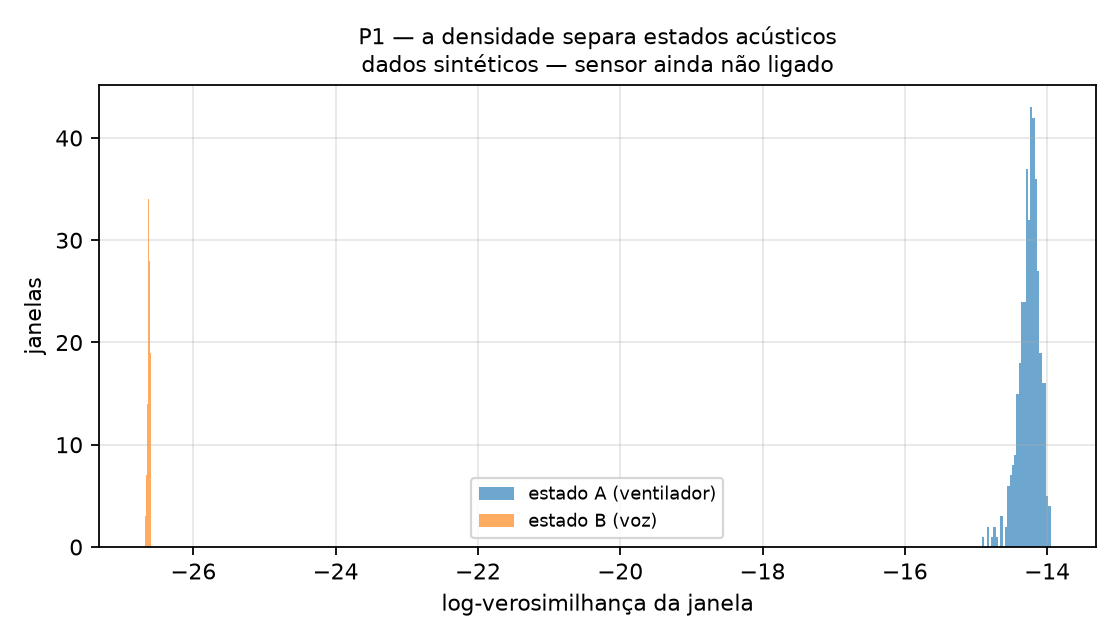
\includegraphics[width=\textwidth]{../figuras/fig2_densidade_por_estado.png}
    \end{column}
  \end{columns}
\end{frame}

\begin{frame}{P2 — o nível seguinte com incerteza}
  \begin{columns}[T]
    \begin{column}{0.48\textwidth}
      \begin{itemize}
        \item Regressão linear bayesiana
        \item Guarda no dispositivo \textbf{7 números}, não os pontos de treino
        \item Variância preditiva: ruído + incerteza nos parâmetros
        \item A banda \textbf{alarga} onde o modelo sabe menos
      \end{itemize}
    \end{column}
    \begin{column}{0.48\textwidth}
      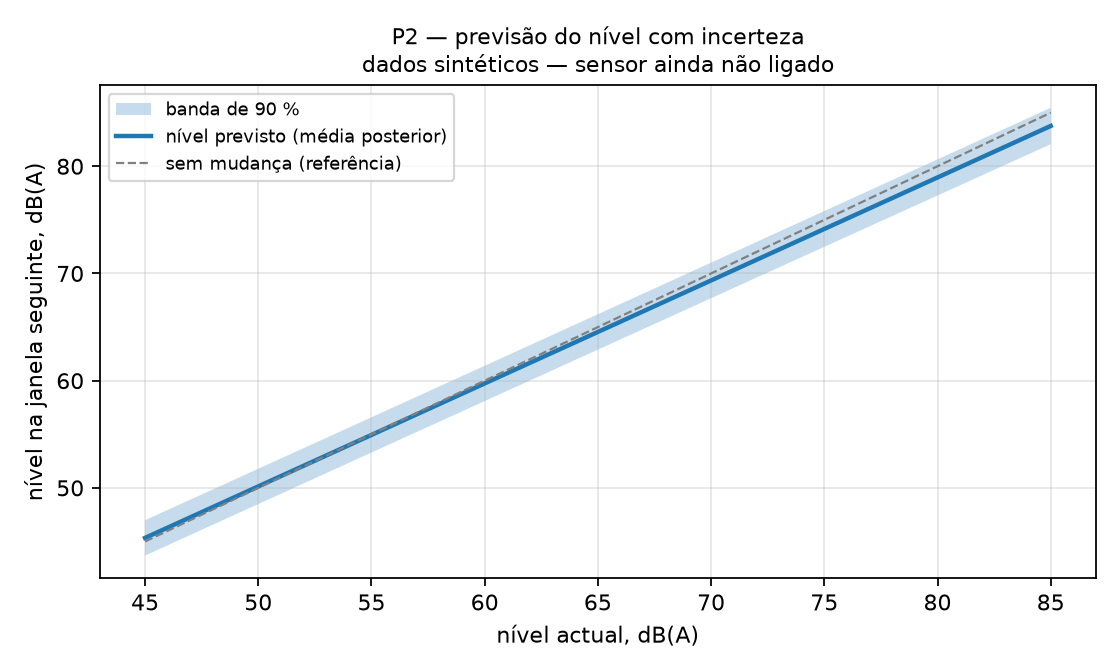
\includegraphics[width=\textwidth]{../figuras/fig1_nivel_com_incerteza.png}
    \end{column}
  \end{columns}
\end{frame}

\begin{frame}{Verificação — testes que podem falhar}
  \begin{block}{Ida-e-volta host $\leftrightarrow$ dispositivo}
    Divergência da log-verosimilhança: $< \num{e-3}$.\\
    \textbf{Controlo:} perturbar as médias em \SI{1}{\decibel} tem de divergir —
    divergiu \num{1.38}. Sem este controlo, o teste compararia o artefacto consigo mesmo.
  \end{block}
  \begin{block}{Cobertura do intervalo}
    Banda de \SI{90}{\percent} exigida a cobrir entre \SI{85}{\percent} e \SI{95}{\percent}.\\
    \textbf{Controlo de largura:} um intervalo de $\pm\SI{0.1}{\decibel}$ tem de cobrir menos
    de \SI{20}{\percent} — se cobrisse \SI{90}{\percent}, o teste não mediria a largura.
  \end{block}
\end{frame}

\begin{frame}{O acelerador MVP — medido, com ressalva}
  \begin{center}
  \begin{tabular}{lrr}
    \toprule
    operação (N=64, fp16) & ciclos & razão \\
    \midrule
    MVP (hardware)  & 289 & \textbf{3,18×} \\
    CPU (laço)      & 921 & \\
    \bottomrule
  \end{tabular}
  \end{center}
  \vspace{0.3cm}
  \begin{alertblock}{Ressalva declarada}
    O laço da CPU soma as palavras como inteiros; o MVP soma \emph{binary16} real. O número da
    CPU é, por isso, \textbf{generoso com a CPU} — o ganho real é maior, não menor.
  \end{alertblock}
  \footnotesize Por medir: MAC com acumulação (faltam codificações de \texttt{sl\_mvp.h}).
\end{frame}

\begin{frame}{RAM e rádio — porque a dose é calculada no dispositivo}
  \begin{center}
  \begin{tabular}{lrl}
    \toprule
    & valor & consequência \\
    \midrule
    1 s @ \SI{303}{kSa/s}, f32 & \SI{1184}{KB} & 4,7× a RAM disponível \\
    1 s @ \SI{16}{kHz}, i16    & \SI{31}{KB}   & cabe 8 s \\
    resultado do dosímetro     & \SI{24}{B/s}  & cabe folgado no BLE \\
    BLE prático                & \SI{127}{KB/s} & 4 × 244 B por 7,5 ms \\
    \bottomrule
  \end{tabular}
  \end{center}
  \vspace{0.3cm}
  A \SI{303}{kSa/s} o rádio precisaria de \SI{592}{KB/s} — 4,7× o que a ligação transporta.
  Áudio cru a \SI{16}{kHz} cabe, mas é \textbf{modo de diagnóstico}, não produto.
\end{frame}

\begin{frame}{O que ainda não está medido}
  \begin{alertblock}{[A MEDIR] — declarado, nunca preenchido com zero}
    \begin{itemize}
      \item captura ritmada por timer a \SI{16}{kHz} exatos (hoje é polled a \SI{303}{kHz})
      \item DPLL para \SI{78}{MHz} (as constantes de tempo mudam com ele)
      \item \SI{60}{s} de notificações a \SI{1}{Hz} sem quedas
      \item dose contra cálculo à mão (a tabela NR-15 ainda não está no crate)
    \end{itemize}
  \end{alertblock}
  \vspace{0.3cm}
  \footnotesize Um zero e um valor não medido parecem iguais num slide — e só um deles é honesto.
\end{frame}

\begin{frame}{Conclusão}
  \begin{block}{O que este trabalho mostra}
    Um dosímetro que reporta incerteza é útil precisamente onde um número isolado falha:
    na decisão de agir ou de medir mais.
  \end{block}
  \begin{itemize}
    \item Os dois modelos exigidos cabem num microcontrolador sem alocador
    \item A correcção é verificável por testes que \emph{podem} falhar
    \item O custo medido decide a arquitectura: \SI{76}{\percent} do núcleo a \SI{303}{kHz}
          contra \SI{18}{\percent} a \SI{16}{kHz}
    \item O acelerador existe e mede-se: \num{3.18}× — com a ressalva declarada
  \end{itemize}
  \vspace{0.3cm}
  \centering \small Obrigado. Perguntas?
\end{frame}

\end{document}
